\documentclass[11pt]{article}

\usepackage[margin=1in]{geometry}
\usepackage{amsmath,amssymb,amsthm,mathtools}
\usepackage{tikz}
\usepackage{tikz-cd}
\usepackage[most]{tcolorbox}
\usepackage{enumitem}
\usepackage{xcolor}
\usepackage[colorlinks=true,linkcolor=blue!50!black,urlcolor=blue!50!black]{hyperref}

% ---------- notation (matches Davis--Kirk) ----------
\newcommand{\Z}{\mathbf{Z}}
\newcommand{\R}{\mathbf{R}}
\newcommand{\RP}{\mathbf{R}P}
\newcommand{\MO}{M_O}
\newcommand{\Mt}{\widetilde{M}}
\newcommand{\Xt}{\widetilde{X}}
\newcommand{\Zpi}{\Z\pi}
\DeclareMathOperator{\Hom}{Hom}
\DeclareMathOperator{\Ext}{Ext}
\DeclareMathOperator{\Aut}{Aut}
\DeclareMathOperator{\im}{im}
\newcommand{\minus}{\smallsetminus}
\newcommand{\iso}{\cong}

% ---------- theorem environments; numbers are typed by hand to match the textbook ----------
\newtheoremstyle{namedit}{\topsep}{\topsep}{\itshape}{}{\bfseries}{.}{.5em}{\thmname{#1}\thmnote{ #3}}
\newtheoremstyle{namedrm}{\topsep}{\topsep}{\normalfont}{}{\bfseries}{.}{.5em}{\thmname{#1}\thmnote{ #3}}
\theoremstyle{namedit}
\newtheorem{thm}{Theorem}
\newtheorem{cor}{Corollary}
\newtheorem{prop}{Proposition}
\newtheorem{lem}{Lemma}
\theoremstyle{namedrm}
\newtheorem{defn}{Definition}
\newtheorem{rem}{Remark}
\newtheorem{ex}{Example}

% ---------- boxes ----------
\newtcolorbox[auto counter]{correction}[1][]{%
  enhanced, breakable,
  colback=red!3, colframe=red!55!black, boxrule=0.6pt,
  fonttitle=\bfseries\small, fontupper=\small,
  left=5pt, right=5pt, top=3pt, bottom=3pt,
  title={Correction \thetcbcounter}, #1}
\newtcolorbox{filled}[1][]{%
  enhanced, breakable,
  colback=gray!6, colframe=gray!55, boxrule=0.5pt,
  fonttitle=\bfseries\small\color{black}, fontupper=\small,
  left=5pt, right=5pt, top=3pt, bottom=3pt,
  title={Filled in}, #1}

\setlist{itemsep=2pt, topsep=4pt}

\title{\vspace{-1.5em}Orientation Double Cover, the Orientation Character,\\
and Twisted Coefficients}
\author{Lecture notes, organized and checked against\\
Davis--Kirk, \emph{Lecture Notes in Algebraic Topology} (2nd ed.), \S\S6.1--6.3}
\date{}

\begin{document}
\maketitle
\vspace{-1.5em}

\noindent\textbf{How to read these notes.}
\begin{itemize}
  \item \textcolor{red!55!black}{\textbf{Red boxes}} mark places where the handwritten notes had a mistake,
        or used a convention that does not match the textbook.
  \item \textcolor{gray}{\textbf{Gray boxes}} mark steps that were left unfinished in the notes and have been filled in.
  \item Theorem numbers follow the textbook. The textbook writes $\MO$ (``O'' for
        \emph{orientation}) for the orientation double cover; the notes wrote $M_0$.
\end{itemize}

\tableofcontents

%======================================================================
\section{Orientations}
%======================================================================

Throughout, $M$ is an $n$-dimensional manifold without boundary. For $x\in M$, excision gives
$H_n(M,M\minus\{x\})\iso H_n(\R^n,\R^n\minus\{0\})\iso\Z$.
For $V\subseteq M$ open and $x\in V$, write
\[
  i_{x,V}\colon (M,\,M\minus V)\hookrightarrow (M,\,M\minus\{x\})
\]
for the inclusion of pairs, and $i_{x,V*}$ for the induced map on $H_n$.

\begin{defn}[6.5 (Orientation)]
An \emph{orientation} of $M$ is a choice of generator $\mu_x\in H_n(M,M\minus\{x\})$ for every
$x\in M$ that \emph{varies continuously}. This means every point has a neighborhood $U$ and a
class $\mu_U\in H_n(M,M\minus U)$ with $i_{x,U*}(\mu_U)=\mu_x$ for all $x\in U$.
\end{defn}

\begin{lem}[1.1 (small balls)]\label{lem:ball}
Let $W\subseteq M$ be a coordinate chart, $W\iso D^n$ (open unit disk), and let
$V=\tfrac12 D^n\subset W$ be the ball of radius $\tfrac12$. Then for every $x\in V$,
\[
  i_{x,V*}\colon H_n(M,M\minus V)\xrightarrow{\ \iso\ } H_n(M,M\minus\{x\})\iso\Z .
\]
\end{lem}

\begin{center}
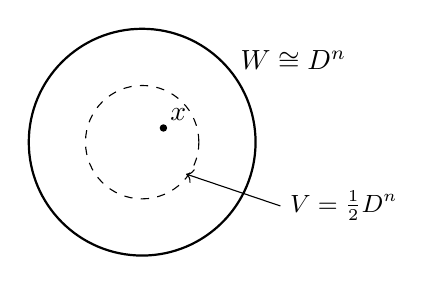
\begin{tikzpicture}[scale=0.9]
  \draw[thick] (0,0) circle (1.6);
  \draw[dashed] (0,0) circle (0.8);
  \fill (0.3,0.2) circle (1.5pt) node[above right=-1pt] {$x$};
  \node[right] at (1.25,1.15) {$W\iso D^n$};
  \draw[->,thin] (1.95,-0.9) node[right] {\small $V=\tfrac12D^n$} -- (0.62,-0.45);
\end{tikzpicture}
\end{center}

\begin{proof}
The closure of $V$ lies in $W$, so excising $M\minus W$ gives
$H_n(M,M\minus V)\iso H_n(D^n,D^n\minus V)$ and
$H_n(M,M\minus\{x\})\iso H_n(D^n,D^n\minus\{x\})$.
Both $D^n\minus V$ and $D^n\minus\{x\}$ deformation retract onto the sphere of radius $\tfrac34$,
so the inclusion $D^n\minus V\hookrightarrow D^n\minus\{x\}$ is a homotopy equivalence. The long
exact sequences of the two pairs and the five lemma finish the proof.
\end{proof}

%======================================================================
\section{The orientation double cover}
%======================================================================

\begin{thm}[6.6]\label{thm:double}
Any $n$-dimensional manifold $M$ has a double cover $p\colon \MO\to M$, where $\MO$ is an
oriented manifold. Moreover, for every $x\in M$, write $p^{-1}(x)=\{x_1,x_2\}$ and let
\[
  \mu_{x_1}\in H_n(\MO,\MO\minus\{x_1\}),\qquad \mu_{x_2}\in H_n(\MO,\MO\minus\{x_2\})
\]
be the local orientations coming from the orientation of $\MO$. Then $p_*(\mu_{x_1})$ and
$p_*(\mu_{x_2})$ are the two generators of $H_n(M,M\minus\{x\})$.
\end{thm}

\begin{correction}[label=c:thm]
The notes call this ``Thm 6.5''. In the textbook it is \textbf{Theorem 6.6}; 6.5 is the definition of
an orientation. The notes also say $\mu_{x_1},\mu_{x_2}$ ``come from [the] orientation of $M$''.
They come from the orientation of $\MO$. The theorem does not assume $M$ is orientable; that is
the whole point.
\end{correction}

\subsection{Construction as a set}
Define
\[
  \MO=\bigl\{(x,a)\;:\;x\in M,\ a\in H_n(M,M\minus\{x\})\text{ is a generator}\bigr\},
  \qquad p(x,a)=x .
\]
Since $H_n(M,M\minus\{x\})\iso\Z$ has exactly two generators $\pm a$, every point of $M$ has exactly
two preimages, $(x,a)$ and $(x,-a)$. (The textbook writes a point of $\MO$ simply as $a$, since
$a$ determines $x$.)

\subsection{Topology}
For $V\subseteq M$ open and $z\in H_n(M,M\minus V)$, set
\[
  V_z=\bigl\{(x,\,i_{x,V*}(z))\;:\;x\in V \text{ and } i_{x,V*}(z)\text{ generates }H_n(M,M\minus\{x\})\bigr\}
  \subseteq \MO .
\]
Topologize $\MO$ by taking $\{V_z\}_{V\subseteq M\text{ open},\ z\in H_n(M,M\minus V)}$ as a basis.
For example, $V_{2u}=\varnothing$ for any $u\in H_n(M,M\minus V)$, because $i_{x,V*}(2u)=2\,i_{x,V*}(u)$ is
never a generator of $\Z$.\footnote{The notes wrote $V_{2w}$. It is renamed here to avoid a clash with
the orientation character $w$ below. The textbook takes $z$ to be a relative cycle in
$Z_n(M,M\minus V)$ rather than a class. Only $[z]$ enters, so the sets $V_z$ are the same.}

\begin{filled}
\textbf{$\{V_z\}$ is a basis.}
\emph{It covers $\MO$:} given $(x,a)$, choose a ball $V\ni x$ as in Lemma~1.1. Since
$i_{x,V*}$ is an isomorphism, there is a unique $z$ with $i_{x,V*}(z)=a$, and then $(x,a)\in V_z$.
\emph{Intersections:} if $(x,a)\in V_z\cap V'_{z'}$, choose a ball $U\ni x$ with $U\subseteq V\cap V'$.
The images of $z$ and $z'$ in $H_n(M,M\minus U)$ both map to $a$ under the isomorphism $i_{x,U*}$, so
they are equal; call this class $z''$. Since $i_{y,V}$ factors through $(M,M\minus U)$ for $y\in U$, we
get $(x,a)\in U_{z''}\subseteq V_z\cap V'_{z'}$.
\end{filled}

\subsection{\texorpdfstring{$p$}{p} is a 2-sheeted covering map}
The notes say: ``$V_z\to V$, $(x,i_{x,V*}(z))\mapsto x$ is locally a bijection; make it a local homeo.''
Here is the precise version.

\begin{prop}[2.1]\label{prop:cover}
The map $p\colon\MO\to M$ has the following properties.
\begin{enumerate}[label=(\alph*)]
  \item For every basic set $V_z$, $p|_{V_z}$ is a homeomorphism onto the open set
        $p(V_z)=\{x\in V: i_{x,V*}(z)\text{ generates}\}$. Hence $p$ is a local homeomorphism.
  \item If $V$ is a ball as in Lemma~1.1 and $z$ generates $H_n(M,M\minus V)\iso\Z$, then
        \[ p^{-1}(V)=V_z\sqcup V_{-z}, \]
        and each piece maps homeomorphically onto $V$.
\end{enumerate}
So $p$ is a 2-sheeted covering map. Since $M$ is a manifold, so is $\MO$.
\end{prop}

\begin{filled}
\textbf{Proof.}
(a) $p|_{V_z}$ is injective, because each $x\in V$ contributes at most one point to $V_z$.
\emph{The image is open:} if $i_{x,V*}(z)$ generates, take a ball $U\ni x$ inside $V$ and let $z_U$ be
the image of $z$ in $H_n(M,M\minus U)$. For $y\in U$ we have $i_{y,V*}(z)=i_{y,U*}(z_U)$, and $i_{y,U*}$ is
an isomorphism. So $i_{y,V*}(z)$ generates if and only if $z_U$ generates, and this holds because it
holds at $y=x$. Hence $U\subseteq p(V_z)$.
\emph{Continuity and openness:} the basic open subsets of $V_z$ are sets $U_{z'}\subseteq V_z$, and their
images are open by what we just showed. Also, for $O\subseteq M$ open,
$p^{-1}(O)\cap V_z=(O\cap V)_{z|}$ is basic open, where $z|$ is the image of $z$ in
$H_n(M,M\minus(O\cap V))$.

(b) For $x\in V$ the map $i_{x,V*}$ is an isomorphism, so $i_{x,V*}(z)$ and $i_{x,V*}(-z)$ are exactly the two
generators of $H_n(M,M\minus\{x\})$. Thus $p^{-1}(V)$ is the disjoint union of $V_z$ and $V_{-z}$, and
$p$ maps each one bijectively, hence homeomorphically by (a), onto $V$.

\emph{$\MO$ is a manifold:} it is locally homeomorphic to $M$. It is Hausdorff: points over different
$x$ are separated by preimages of disjoint open sets in $M$, and $(x,a)$, $(x,-a)$ are separated by
$V_z$ and $V_{-z}$. \qed
\end{filled}

\subsection{The orientation of \texorpdfstring{$\MO$}{M\_O}}

Fix $(x,a)\in\MO$. Choose an open $\widetilde D\ni(x,a)$ so small that $p$ maps $\widetilde D$
homeomorphically onto a ball $D\subseteq M$. Then there is a chain of canonical isomorphisms
\[
  H_n\bigl(\MO,\MO\minus\{(x,a)\}\bigr)
  \;\overset{\text{exc}}{\iso}\;
  H_n\bigl(\widetilde D,\widetilde D\minus\{(x,a)\}\bigr)
  \;\overset{(p|_{\widetilde D})_*}{\iso}\;
  H_n\bigl(D,D\minus\{x\}\bigr)
  \;\overset{\text{exc}}{\iso}\;
  H_n\bigl(M,M\minus\{x\}\bigr).
\]
Call the composite $p_*$. It does not depend on $\widetilde D$, because any two choices contain a
smaller common one.

\begin{defn}
Let $\mu_{(x,a)}\in H_n(\MO,\MO\minus\{(x,a)\})$ be the generator that corresponds to $a$, that is,
$p_*(\mu_{(x,a)})=a$.
\end{defn}

\begin{correction}[label=c:excision]
The notes wrote $H_n(\MO,\MO\minus\{(x,a)\})\iso H_n(D^n,D^n\minus\tfrac12D^n)$ ``by excision''.
Excision only shrinks the ambient space. The second group in the pair stays a \emph{point}
complement, as in the chain above. The ball complement $H_n(-,-\minus\tfrac12D^n)$ is the group used
to check continuity (see the next box), not the local homology at a point.\par\smallskip
Also note that $p$ does \emph{not} map $\MO\minus\{(x,a)\}$ into $M\minus\{x\}$, since
$(x,-a)\mapsto x$. So ``$p_*$'' in Theorem~6.6 has to mean the composite above. It is not
induced by a map of pairs.
\end{correction}

\begin{filled}
\textbf{Why $\{\mu_{(x,a)}\}$ is an orientation (varies continuously).}
Given $(x,a)$, take a ball $V\ni x$ and $z\in H_n(M,M\minus V)$ with $i_{x,V*}(z)=a$. Take a smaller
ball $V'\ni x$ whose closure lies in $V$, and set $\widetilde V'=V'_{z|}\subseteq V_z$. Since
$p\colon V_z\to V$ is a homeomorphism, excision gives
\[
  H_n(\MO,\MO\minus\widetilde V')\iso H_n(V_z,V_z\minus\widetilde V')\iso H_n(V,V\minus V')\iso H_n(M,M\minus V').
\]
Let $\tilde z$ be the class corresponding to the image of $z$. By naturality, $\tilde z$ restricts to
$\mu_{(y,\,i_{y,V*}(z))}$ at every point of $\widetilde V'$. This is exactly the condition in
Definition~6.5.
\end{filled}

\begin{proof}[Proof of the ``moreover'' part of Theorem~6.6]
We have $p^{-1}(x)=\{(x,a),(x,-a)\}$, and by construction
\[
  p_*(\mu_{(x,a)})=a,\qquad p_*(\mu_{(x,-a)})=-a,
\]
which are the two generators of $H_n(M,M\minus\{x\})$.
\end{proof}

\subsection{The deck transformation}
$p\colon\MO\to M$ is a principal $\Z/2$-bundle. Write $\Z/2=\{1,T\}$: the element $1$ acts as the
identity and $T$ switches the two points of each fiber,
\[
  T(x,a)=(x,-a).
\]
$T$ is a homeomorphism because $T(V_z)=V_{-z}$. Also $p\circ T=p$, and $T$ acts freely with quotient $M$.

\begin{rem}
$T$ \emph{reverses} the orientation of $\MO$. Since $p\circ T=p$, we have
$p_*T_*\mu_{(x,a)}=p_*\mu_{(x,a)}=a=-p_*\mu_{(x,-a)}$. Hence $T_*\mu_{(x,a)}=-\mu_{T(x,a)}$.
\end{rem}

\subsection{Examples}
\begin{itemize}
  \item \textbf{$M$ orientable} (and connected) with orientation $\mu$:
        \[ \MO=(M,\mu)\sqcup(M,-\mu), \]
        with sheets $\{(x,\mu_x)\}$ and $\{(x,-\mu_x)\}$, each mapping homeomorphically onto $M$.
  \item \textbf{$M$ non-orientable:} e.g.\ $S^n\to\RP^n$ for $n$ \emph{even}. The deck transformation
        is the antipodal map, which has degree $(-1)^{n+1}=-1$ and so reverses orientation, as the
        remark predicts.
\end{itemize}

\begin{correction}[label=c:rpn]
The notes give $S^n\to\RP^n$ as the example with no restriction on $n$. This is the orientation
double cover only for \textbf{$n$ even}. For $n$ odd, $\RP^n$ is orientable, and its orientation double
cover is $\RP^n\sqcup\RP^n$ with opposite orientations (textbook, p.~150).
\end{correction}

%======================================================================
\section{The orientation character}
%======================================================================

\begin{defn}[(Orientation character)]
Let $M$ be a connected manifold with base point $m_0$. The \emph{orientation character} of $M$, also
called the \emph{first Stiefel--Whitney class}, is
\[
  w\colon\pi_1(M,m_0)\to\{\pm1\},\qquad
  w([\gamma])=
  \begin{cases}
    \ \ 1 & \text{if }\gamma\text{ lifts to a closed loop in }\MO,\\
    -1 & \text{otherwise.}
  \end{cases}
\]
Equivalently, the lift of $\gamma$ starting at $(m_0,a)$ ends at $(m_0,\,w[\gamma]\,a)$. Intuitively,
$w[\gamma]=-1$ when carrying the local orientation around $\gamma$ reverses it.
\end{defn}

\begin{filled}
\textbf{$w$ is well defined and a homomorphism.} (The notes break off at ``well defined b/c\ldots''.)
\begin{itemize}
  \item \emph{It does not depend on the representative $\gamma$:} by the homotopy lifting property,
        loops that are homotopic rel endpoints have lifts with the same endpoint when started at the
        same point.
  \item \emph{It does not depend on which preimage of $m_0$ we start at:} the other lift is
        $T\circ\tilde\gamma$, which is closed exactly when $\tilde\gamma$ is.
  \item \emph{It is a homomorphism:} the lift of $\gamma$ from $(m_0,a)$ ends at $(m_0,w(\gamma)a)$.
        The lift of $\delta$ from there ends at $(m_0,w(\delta)w(\gamma)a)$, using $T$ when
        $w(\gamma)=-1$. So $w(\gamma\delta)=w(\gamma)w(\delta)$.
\end{itemize}
\end{filled}

\begin{prop}[3.1]\label{prop:orient}
Let $M$ be connected. Then $M$ is orientable if and only if $w\equiv1$.
\end{prop}

\begin{proof}
The notes give the key reason: $M$ is orientable $\iff$ $\MO\iso M\sqcup M$. In more detail, an
orientation of $M$ is the same thing as a continuous section $x\mapsto(x,\mu_x)$ of $p$; continuity
of the section is exactly ``varies continuously'', by the definition of the $V_z$ topology. For
connected $M$, a double cover has a section if and only if it is trivial, $\MO\iso M\times\{\pm1\}$.
That happens if and only if every loop at $m_0$ lifts to a loop, that is, $w\equiv1$.
\end{proof}

\begin{correction}[label=c:sqcup]
``$\MO=M\sqcup M$'' should be read as an isomorphism \emph{of covering spaces} over $M$ (the cover
is trivial), and the statement needs $M$ connected. For connected $M$ this is the same as saying
$\MO$ is disconnected.
\end{correction}

\begin{cor}[6.7]
If $H^1(M;\Z/2)=0$, then $M$ is orientable.
\end{cor}

\begin{proof}
We may assume $M$ is connected: $M$ is orientable if and only if each component is, and $H^1$ of $M$
is the product of $H^1$ of its components. By the universal coefficient theorem,
\[
  H^1(M;\Z/2)\;\iso\;\Hom(H_1M,\Z/2)\oplus\Ext(H_0M,\Z/2)\;=\;\Hom(H_1M,\Z/2),
\]
because $H_0M\iso\Z$ is free, so the $\Ext$ term vanishes. The Hurewicz theorem gives
$H_1M\iso\pi_1M/[\pi_1M,\pi_1M]$, and since $\Z/2$ is abelian, every homomorphism
$\pi_1M\to\Z/2$ factors uniquely through the abelianization. Hence
\[
  H^1(M;\Z/2)\;\iso\;\Hom\bigl(\pi_1M/[\pi_1M,\pi_1M],\,\Z/2\bigr)\;=\;\Hom(\pi_1M,\Z/2).
\]
So if $H^1(M;\Z/2)=0$, every homomorphism $\pi_1M\to\Z/2$ is trivial. In particular
$w\colon\pi_1M\to\{\pm1\}\iso\Z/2$ is trivial, and $M$ is orientable by
Proposition~3.1.
\end{proof}

\begin{correction}[label=c:uct]
The notes start the proof with $H^1(M;\Z)\overset{\text{UCT}}{\iso}\Hom(H_1(M),\Z/2)\oplus\cdots$. The
left side should be $H^1(M;\Z/2)$. The term $\Ext(H_0(M),\Z/2)$, which is crossed out in the notes,
belongs in the UCT. It is zero because $H_0(M)$ is free. The Hurewicz step needs $M$ connected, which
is why we reduced to that case first.
\end{correction}

\begin{rem}
The converse fails. For example, the torus $T^2$ is orientable but $H^1(T^2;\Z/2)\iso(\Z/2)^2$.
\end{rem}

%======================================================================
\section{Homology with twisted coefficients}
%======================================================================

\subsection{Conventions (textbook \S6.1)}
Let $X$ be path-connected and locally path-connected, with universal cover $\Xt$, and set
$\pi=\pi_1(X,x_0)$. In the textbook, $\pi$ acts on $\Xt$ on the \emph{right} by covering
transformations (as for a principal $\pi$-bundle). So $S_*(\Xt)$ is a right $\Zpi$-module, with
$\sigma\cdot g$ the composite of $\sigma$ and the covering transformation $g$. A homomorphism
$\rho\colon\pi\to\Aut(A)$ makes the abelian group $A$ a \emph{left} $\Zpi$-module:
\[
  \Bigl(\sum m_g\,g\Bigr)\cdot a=\sum m_g\,\rho(g)(a).
\]

\begin{defn}[6.3 and 6.4]
\[
  H_*(X;A_\rho)=H_*\bigl(S_*(\Xt)\otimes_{\Zpi}A\bigr),\qquad
  H^*(X;A_\rho)=H^*\bigl(\Hom_{\Zpi}(S_*(\Xt),A)\bigr).
\]
For the $\Hom$, $S_*(\Xt)$ is turned into a left module by $g\cdot z:=z\cdot g^{-1}$.
\end{defn}

\begin{correction}[label=c:sides]
The notes write: ``If $\pi_1X$ acts on $A$ on the right via $\rho\colon\pi_1X\to\Aut A$, then
$H_*(X;A_\rho)=H_*(A\otimes_{\Z[\pi_1X]}S_*(\Xt))$ and
$H^*(X;A_\rho)=H^*(\Hom_{\Z[\pi_1X]}(S_*(\Xt),A))$.'' Two consistency issues:
\begin{enumerate}[label=(\roman*)]
  \item A homomorphism $\rho$ naturally gives a \emph{left} action $g\cdot a=\rho(g)(a)$. To get a right
        action you set $a\cdot g:=\rho(g^{-1})(a)$.
  \item A tensor product pairs a right module with a left module, but $\Hom_{\Zpi}$ needs both modules
        on the \emph{same} side. If $A$ is a right module in $A\otimes S_*(\Xt)$, then $S_*(\Xt)$ must be
        a left module there, and then $\Hom_{\Zpi}(S_*(\Xt),A)$ pairs a left module with a right one.
\end{enumerate}
The notes' formulas are the mirror image of the textbook's and give the same groups once the sides are
converted consistently with $g\leftrightarrow g^{-1}$. These notes use the textbook's convention.
\end{correction}

\subsection{The orientation coefficient system \texorpdfstring{$\Z_w$}{Z\_w}}
Since $\Aut(\Z)=\{\pm1\}$, the orientation character is a representation
$w\colon\pi_1M\to\{\pm1\}=\Aut(\Z)$. Write $\Z_w$ for $\Z$ with $g\cdot m=w(g)\,m$. The groups
\[
  H_*(M;\Z_w),\qquad H^*(M;\Z_w)
\]
are the (co)homology of $M$ \emph{twisted by the orientation character}, or with \emph{local
coefficients in the orientation sheaf}.

\paragraph{As a bundle of groups.}
The corresponding local coefficient system is the balanced product
\[
  E_w=\Mt\times_{\pi}\Z_w=(\Mt\times\Z)\big/\bigl((\tilde m g,\,m)\sim(\tilde m,\,g m)\bigr)\longrightarrow M .
\]
\begin{itemize}
  \item If $M$ is \textbf{orientable}, then $w$ is trivial and $E_w\iso M\times\Z$ is the trivial bundle.
  \item If $M$ is \textbf{non-orientable} (and connected), then $\ker w=p_*\pi_1(\MO)$ has index 2,
        $\Mt/\ker w\iso\MO$, and the deck group is $\pi/\ker w\iso\Z/2=\{1,T\}$. Since $\ker w$ acts
        trivially on $\Z_w$,
        \[ E_w\iso\MO\times_{\Z/2}\Z_-, \]
        where $T$ acts on $\Z$ by $-1$.
\end{itemize}
In fact $E_w\iso\MO\times_{\Z/2}\Z_-$ in both cases, since for orientable $M$ the right side is
$M\times\Z$. It is also the orientation sheaf $\bigcup_{x}H_n(M,M\minus\{x\})$ of textbook \S6.3, and
$\MO$ sits inside it as the elements $\pm1$ of each fiber.

\begin{correction}[label=c:bundle]
The notes wrote ``$\Z\times_{\pi_1}\Mt$; $M$ oriented: get $\Z\times M$; $M$ not oriented:
$M\times_{\Z/2}M_0$'' (the last formula is hard to read). The fixes:
\begin{itemize}
  \item The textbook writes $\Mt\times_\pi\Z_w$, since $\pi$ acts on $\Mt$ on the right and on $\Z$ on
        the left.
  \item ``Oriented'' should be ``orientable'': $w$ depends only on whether an orientation exists.
  \item In the non-orientable case the bundle is $\MO\times_{\Z/2}\Z_-$.
\end{itemize}
\end{correction}

%======================================================================
\section{Poincar\'e duality with twisted coefficients}
%======================================================================

\subsection{Products with coefficients}
A bilinear pairing of coefficients $R\times S\to P$ induces cup and cap products (textbook
Exercise~61 and pp.~103--104):
\[
  \cup\colon H^p(X;R)\times H^q(X;S)\to H^{p+q}(X;R\otimes S),\qquad
  \cap\colon H^q(X;R)\times H_{p+q}(X;S)\to H_p(X;P).
\]
With twisted coefficients the pairing has to be $\pi$-equivariant, where $R\otimes S$ carries the
diagonal action $g(r\otimes s)=gr\otimes gs$.\footnote{The textbook only sketches products with local
coefficients (its margin note reads ``Add discussion of cup and cap products with local
coefficients''). The equivariance requirement is the standard one.}
The point in the notes is that multiplication gives the two equivariant pairings we need:
\[
  \Z_w\otimes\Z_w\to\Z,\qquad \Z_w\otimes\Z\to\Z_w,\qquad m\otimes m'\mapsto mm'.
\]
These are equivariant because $w(g)m\cdot w(g)m'=w(g)^2mm'=mm'$, so the action on $\Z_w\otimes\Z_w$ is
trivial, and $w(g)m\cdot m'=w(g)\,mm'$.

\subsection{The theorem}

\begin{thm}[6.8 (Poincar\'e duality)]
Let $X$ be an $n$-dimensional manifold that is connected, compact, and without boundary. Then
\[
  H_n(X;\Z_w)\iso\Z,
\]
and if $[X]$ denotes a generator, then
\[
  \cap[X]\colon H^k(X;\Z_w)\xrightarrow{\ \iso\ }H_{n-k}(X;\Z)
  \qquad\text{and}\qquad
  \cap[X]\colon H^k(X;\Z)\xrightarrow{\ \iso\ }H_{n-k}(X;\Z_w)
\]
are isomorphisms. This applies to non-orientable as well as orientable manifolds.
\end{thm}

\begin{rem}
The cap products come from the pairings above, with $[X]\in H_n(X;\Z_w)$:
\[
  H^k(X;\Z_w)\times H_n(X;\Z_w)\to H_{n-k}(X;\Z_w\otimes\Z_w)=H_{n-k}(X;\Z),
\]
\[
  H^k(X;\Z)\times H_n(X;\Z_w)\to H_{n-k}(X;\Z\otimes\Z_w)=H_{n-k}(X;\Z_w).
\]
If $X$ is orientable, then $w\equiv1$ and $\Z_w=\Z$, and both statements reduce to ordinary Poincar\'e
duality (Theorem~4.29) with $[X]$ the fundamental class.
\end{rem}

%======================================================================
\section{Invariants and coinvariants}
%======================================================================

\begin{defn}
Let $A$ be an abelian group, and let a group $G$ act on $A$ through $\Aut(A)$, i.e.\ via a homomorphism
$\rho\colon G\to\Aut(A)$.
\begin{itemize}
  \item The \emph{$G$-invariants} of the action are
        \begin{align*}
          A^G&=\{a\in A: ga=a\ \ \forall g\in G\} && \text{(left action)},\\
          A^G&=\{a\in A: ag=a\ \ \forall g\in G\} && \text{(right action)}.
        \end{align*}
  \item The \emph{$G$-coinvariants} are
        \begin{align*}
          A_G&=A\big/\langle\,ga-a: g\in G,\ a\in A\,\rangle && \text{(left action)},\\
          A_G&=A\big/\langle\,ag-a: g\in G,\ a\in A\,\rangle && \text{(right action)}.
        \end{align*}
\end{itemize}
So $A^G$ is the largest subgroup on which $G$ acts trivially, and $A_G$ is the largest quotient on which
$G$ acts trivially. Equivalently, $A_G\iso\Z\otimes_{\Z G}A$ and $A^G\iso\Hom_{\Z G}(\Z,A)$, with $\Z$ the
trivial module.
\end{defn}

\begin{filled}
The notes leave ``for right \underline{\quad}'' blank in both definitions; the right-action versions are
filled in above.
\end{filled}

\begin{prop}[6.9 (from the textbook; where this is going)]
Let $X$ be path-connected, $\pi=\pi_1(X,x_0)$, and $A$ a left $\Zpi$-module. Then
\[
  H_0(X;A)\iso A_\pi,\qquad H^0(X;A)\iso A^\pi .
\]
\end{prop}

\begin{ex}[(sanity check: Proposition 6.9 together with Theorem 6.8)]
Let $X$ be closed, connected, and non-orientable, so $w$ is nontrivial. Then
\[
  (\Z_w)^\pi=\{m: -m=m\}=0,\qquad (\Z_w)_\pi=\Z/\langle m-(-m)\rangle=\Z/2 .
\]
Poincar\'e duality gives $H_n(X;\Z)\iso H^0(X;\Z_w)=0$ and $H^n(X;\Z)\iso H_0(X;\Z_w)=\Z/2$. These
agree with the familiar facts for closed non-orientable manifolds; for example,
$H_2(\RP^2;\Z)=0$ and $H^2(\RP^2;\Z)=\Z/2$.
\end{ex}

%======================================================================
\section*{Summary of corrections}
\addcontentsline{toc}{section}{Summary of corrections}
%======================================================================
\begin{enumerate}[label=\textbf{\arabic*.}, leftmargin=2em]
  \item (Correction~\ref{c:thm}) The double cover theorem is Theorem \textbf{6.6} in the textbook. The
        orientations $\mu_{x_i}$ come from the orientation of $\MO$, not of $M$.
  \item (Correction~\ref{c:excision}) Excision gives the \emph{point} complement
        $H_n(\widetilde D,\widetilde D\minus\{(x,a)\})$, not $H_n(D^n,D^n\minus\tfrac12D^n)$. The map
        ``$p_*$'' on local homology is a composite of isomorphisms, not a map of pairs.
  \item (Correction~\ref{c:rpn}) $S^n\to\RP^n$ is the orientation double cover only for $n$ even. For $n$
        odd it is $\RP^n\sqcup\RP^n$.
  \item (Correction~\ref{c:sqcup}) ``$\MO=M\sqcup M$'' means the cover is trivial, i.e.\ an isomorphism of
        covering spaces, and needs $M$ connected.
  \item (Correction~\ref{c:uct}) In Corollary 6.7, $H^1(M;\Z)$ should be $H^1(M;\Z/2)$. The $\Ext$ term
        belongs in the UCT and vanishes because $H_0$ is free.
  \item (Correction~\ref{c:sides}) Twisted coefficients: the module sides in the notes' $\otimes$ and $\Hom$
        formulas don't match each other. Use the textbook's $S_*(\Xt)\otimes_{\Zpi}A$ and
        $\Hom_{\Zpi}(S_*(\Xt),A)$ with $A$ a left module.
  \item (Correction~\ref{c:bundle}) The coefficient bundle is $\Mt\times_\pi\Z_w\iso\MO\times_{\Z/2}\Z_-$.
        ``Oriented'' should be ``orientable''.
\end{enumerate}
Gaps filled in: the basis property of $\{V_z\}$; $p$ as a covering map; continuity of the orientation on
$\MO$; well-definedness of $w$ (the notes break off there); and the right-action versions of
invariants and coinvariants.

\end{document}
